\subsection{Stochastic Volatility}\label{ssec:stochastic_volatility}

\begin{figure*}[t]
    \centering
    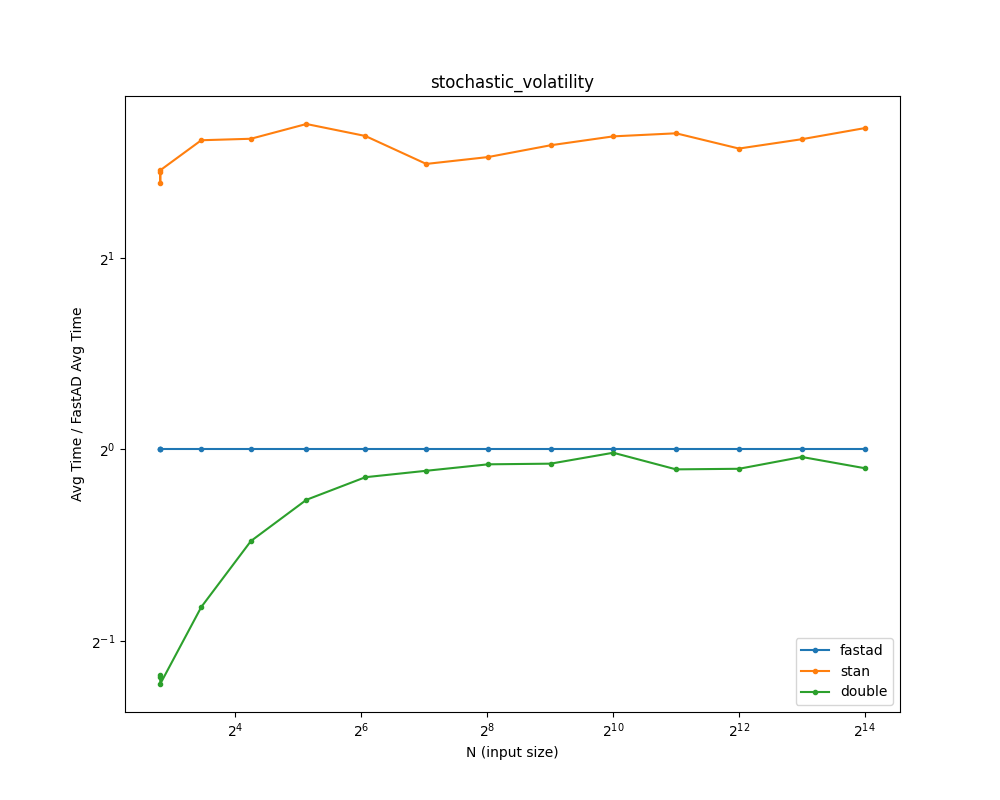
\includegraphics[width=0.8\textwidth]{figs/stochastic_volatility_fig.png}
    \caption{%
        Stochastic volatility benchmark of Stan against FastAD 
        plotted relative to FastAD average time.
    }\label{fig:stochastic_volatility}
\end{figure*}

This section marks the second and last macro-benchmark example.
We consider the following stochastic volatility model 
taken from the Stan user guide~\cite{stan-rm:2018}:
\begin{align*}
    y &\sim N(0, e^{h}) \\
    h_{std} &\sim N(0, 1) \\
    \sigma &\sim Cauchy(0,5) \\
    \mu &\sim Cauchy(0,10) \\
    \phi &\sim Unif(-1, 1) \\
    h &= h_{std} \cdot \sigma \\
    h[0] &= \frac{h[0]}{\sqrt{1 - \phi^2}} \\
    h &= h + \mu \\
    h[i] &= \phi \cdot (h[i-1] - \mu),\, i > 0
\end{align*}
The target function is the log of the joint probability density function (up to a constant)
and we wish to differentiate it with respect to $h_{std}, h, \phi, \sigma, \mu$.
For this benchmark, we only consider Stan for the same reasons described in Section~\ref{ssec:regression}.
The fill function for this functor will resize a vector of size $N$ as $\tilde{N} = N + 3$,
where the first $N/2$ values refer to $h_{std}$,
the next $N/2$ values refer to $h$,
and the next three refer to $\phi, \sigma, \mu$, respectively.
We take care of the edge case where $N < 2$ to let $N = 2$ and then carry out the steps above.
Here, $y$ is a constant.
All quantities are randomly generated uniformly in $(-1,1)$ range
and $\sigma$ is modified afterwards to be strictly positive.
Fig.\ref{fig:stochastic_volatility} shows the benchmark results.

FastAD outperforms Stan by 3 times for the largest $N$.
The trend seems quite stabilized from the start.
It is interesting to see that FastAD is only marginally slower than the \code{double} baseline
for moderate to large $N$ values.
The ratio between FastAD time to baseline time is $ 1.07$, which means there is about a $7\%$ overhead 
just from one \emph{forward-evaluation} to \emph{also} compute the gradient.
Hence, gradient computation is almost free from just computing the log-pdf,
which puts FastAD at near-optimal performance.
